\documentclass[english,bachelor,a4paper,oneside]{ppfcmthesis}

\usepackage[utf8]{inputenc}
\usepackage[OT4]{fontenc}

% Authors here.
\author{%
   Kamil Kołodziej \album{127272} \and 
   Kinga Neumann \album{127224} \and 
   Miłosz Pogodski \album{127206} \and 
   Patryk Stasiewski \album{127281}}
\title{NVM-enabled Distributed Hash Table system}
\ppsupervisor{Ph.D.~Tadeusz Kobus, MSc.~Maciej Kokociński}

\ppyear{2019}                                         

\begin{document}

% Front matter starts here
\frontmatter\pagestyle{empty}%
\maketitle\cleardoublepage%

% Blank info page for "karta dyplomowa"
\thispagestyle{empty}\vspace*{\fill}%
\begin{center}Tutaj przychodzi karta pracy dyplomowej;\\oryginał wstawiamy do wersji dla archiwum PP, w pozostałych kopiach wstawiamy ksero.\end{center}%
\vfill\cleardoublepage%

% Table of contents.
\pagenumbering{Roman}\pagestyle{ppfcmthesis}%
\tableofcontents* \cleardoublepage%

% Main content of your thesis starts here.
\mainmatter%
\chapter{Introduction} \label{Introduction}

\section{Motivations}

Traditional computers use two types of memories: Random Access Memory (RAM) for direct data access and Solid-State or Hard-Disk Drives (SSD, HDD) for its long-term storage. Although RAM enables quick access to memory, the data it stores are volatile and hence are lost after each system shutdown. On the other hand, both SSDs and HDDs provide persistent storage but at the cost of much higher access latency compared to RAM.

Recently one can observe the emergence of a new technology called \emph{Non-Volatile Memory} (NVM) (sometimes also referred to as \emph{Persistent Memory}, PM). NVM is aimed as a replacement for both RAM and disks by combining their best features. NVM promises high throughput, low latency and byte addressability, similarly to RAM, but it will also guarantee data persistence in case of power outage \cite{NvmPerformanceArticle}. 

NVM creates new possibilities as well as many challenges in the IT sector. Incorporating NVM will result in significant improvements in the performance of computer systems. It is because storing and retrieving large amounts of data will happen much more quickly. Moreover, thanks to NVM, complex services running on the Internet will not require complicated caching mechanisms to overcome the performance limitations of the traditional data storage solutions. NVM will also ease the process of recovery after computer crashes, i.e., providing data durability will be straightforward and the time consuming process of loading data from disks to memory upon recovery will not be necessary any longer. Therefore, one can expect that the use of NVM will particularly beneficial in distributed systems, which often feature crash recovery procedures that heavily rely on the synchronous access to the stable storage. 

However, leveraging the capabilities of NVM means that a new approach to designing and implementing applications is needed. In particular, memory has to be carefully allocated so no memory leaks occur when the application crashes. For the similar reason, write operations to NVM must be properly managed in order to ensure that the data kept in memory is always consistent.

\section{Goal}

The main goal of the following thesis was to design, implement and test the \textbf{NVM-enabled distributed hash table system} and thus to evaluate the benefits and costs of using NVM to create a highly available distributed application. 
The design of our system, which is called \DHTS, follows the principles of Amazon Dynamo \cite{AmazonDynamo}. It means that the system is composed of multiple nodes, each of which has similar responsibilities (there is no central coordinator) and that the system can easily scale horizontally by adding new nodes to it. Nodes communicate using a gossip protocol. For durability, each node stores data in a custom-built NVM-enabled hash table called \emph{Persistent Hash Table (\PHT)}. In order to provide high availability data is additionally replicated across multiple nodes. The level of data replication is tunable via a configuration parameter.

In order to build \PHT, our local NVM-enabled hash table, we relied on \emph{Persistent Memory Development Kit} \cite{PmemIo}, a set of libraries and tools provided by Intel for NVM. NVM is a new technology and although some NVM hardware is already available on the market, we did not have access to it. Therefore, we opted for NVM emulation using RAM.

We developed a range of tests to evaluate the performance independently for \PHT and \DHTS. The tests results of \PHT show the inherent overhead introduced by using NVM to manage data: accessing and modifying data stored in NVM is 2-10 times slower compared to similar operations performed on volatile RAM. Moreover, NVM requires that some metadata are stored alongside data. The memory overhead is caused by the fact that in NVM libraries memory has to be allocated in blocks of fixed size. 

We deployed \DHTS on the HPC cluster available at the faculty's premises. The test results indicate that the system scales well with the increasing number of nodes.

\section{Thesis structure}

The structure of the thesis is as follows. In Chapter~\ref{Background} we discuss NVM in more detail and we describe tools and libraries used implementing \DHTS. We discuss the implementation details and the evaluation of \PHT in Chapter~\ref{OwnWork}. The design and implementation of \DHTS is given in Chapter~\ref{Distribution}. We conclude in Chapter~\ref{Conclusion}.

\bigskip

\noindent Below we outline the roles of each co-author in this project:
\begin{itemize}
    \item Patryk Stasiewski -- the configuration of the \NVM programming environment, the design and implementation of \emph{\PersistentHashTable},
    \item Kinga Neumann -- the design and implementation of \emph{\PersistentHashTable}, the development of unit tests of \emph{\PersistentHashTable},
    \item Kamil Kołodziej -- the configuration of the virtualization environment using Docker, the design and implementation of \DHTS,
    \item Miłosz Pogodski -- the design and implementation of \DHTS, tests of \DHTS.
\end{itemize}

\chapter{Background} \label{Background}

In this chapter we will discuss concepts and technologies used to develop our system.

\section{Non-Volatile Memory and Persistent Memory}
    

    \subsection{Definitions}
        \NVM (NVM) is a class of memory storage devices which are able to keep data after power outage. Consequently, they are suitable for systems which rely on data durability, such as database systems.
        Nowadays a noticable drawback of this type of memory is a fact that it is much slower than their volatile counterparts.  
        Currently high-performance NVM solutions are expensive and offer low capacity while still having a significant lack of performance in comparison to DRAM memory. 
        The performance of NVM, however, is still improving and the gap between NVM and DRAM is expected to be insignificant in the future. 
        
        \PM (PM) is a byte-addressable, non-volatile memory which can be directly accessed via the memory bus.
        
    \subsection{Access to NVM}
        %\tk{Correct me if I'm wrong, but it seems to me that at least Intel uses the same technology to created PM as well as for a new kind of SSDs, which are treated by the operating system as block devices (Intel Optane?).}
    
        In most computer applications access to data storage proceeds as follows:
        \begin{itemize}
            \item Application uses the file system API to access the files.
            \item File system performs read and write operations through a driver.
            \item All data transferred during those operations is composed of blocks, typically of size 4KB.
        \end{itemize}
        The solution described above is inadequate from the point of view of PM, because it makes programmers unable to utilise the low latency byte-addressable direct access supported by the hardware.
        To solve this issue the support for \DAX (DAX) mode was incorporated into operating systems.
        In this approach persistent memory-aware file system is used to map virtual addresses to physical addresses in PM \cite{PmemAccess}. 
        It allows applications to directly access individual bytes of the storage without the necessity to operate on entire blocks. By memory-mapping files located in the file system present in the PM, the processes attach a region of persistent memory to their address space and simply use it as an ordinary operating memory  segment.
      
    \subsection{Emulation}
        NVM hardware is not yet easily available and during this project we were not able obtain an access to it. However, in order to build and test NVM-enabled applications, it is possible to emulate the hardware by marking segments of ordinary RAM as persistent and creating a DAX-enabled file system on them \cite{PmemEmulation}.
        % Emulation is based on DRAM memory, which is recognised by operating system as persistent memory region.
        Such an environment, which we call \emph{emulated Persistent Memory}, naturally will not keep data after power outage, but it will provide performance comparable to the performance of the envisioned NVM hardware solutions. Alternatively, regular stable storage could be used for emulation, but such an approach would induce severe performance penalty. 
        
    \subsection{Developing applications for NVM}
        
        %\tk{This subsection requires more details. Why do we get corrupted or incomplete data? Why a mutex won't be released? Because after a crash, the state of processes/threads is not restored. Processes operate in RAM, cache and processor registers, the contents all of which can be lost event though NVM is used. Maybe give an example of what might happen. }
    
        Programming for persistent memory differs from programming for volatile memory. 
        In case of this project there are two most important differences that should be considered.
        
        Firstly, persistent memory is not reinitialised after the application restart. It implies that a data structure kept in PM might include some corrupted or incomplete data, which in turn may result in the program crash or some incorrect and unexpected behaviour. Such situations may occur when an application is aborted, by user interaction or by exception coming from other thread, when performing write operation to memory. In that case, data will be saved only partially. To prevent such situations a transactional mechanism can be employed (as in the \libpmemobj library, which we use to access NVM, see Chapter~\ref{OwnWork}). Then all writes to NVM are performed within a transaction, which guarantees that they will be executed atomically.
        
        Secondly, using persistent memory together with mutexes for inter-thread synchronisation may lead to unintended behaviour. 
        For processes which operate in RAM, a mutex is stored in the volatile memory. When that process terminates, memory allocated by the process is released, so upon the subsequent execution the mutex will be reinitialised and set to unlocked. When a process operates in non-volatile memory and terminates when the mutex is locked, its state is kept in persistent memory. When the process
        restarts, the mutex will not be reinitialised and will be still locked. As a consequence, when a thread crashes after locking a mutex stored in NVM, it may never unlock which results in a deadlock. To solve that problem there is a special type of NVM-aware mutexes which are stored in the persistent memory, but are reinitialised on the program startup when necessary. 
      
\section{Persistent Memory Development Kit}

    \subsection{Overview}
        Persistent Memory Development Kit (PMDK) \cite{PmemIo} is a set of tools and libraries developed by Intel Corporation, whose aim is to support persistent memory programming. It is based on memory-mapped files (POSIX \texttt{mmap} system call). PMDK consists of 10 libraries suitable for various tasks, most important of which are described below. It also features extensive documentation, which includes examples that demonstrate how to use each of those libraries. We discuss our usage of those libraries in the next chapter.
        
    \begin{enumerate}
    
    \item
        \texttt{libpmem} -- a library which provides a low-level persistent memory API for C language. It requires developers to handle memory allocation and flush changes to persistent memory by themselves. It also does not provide transactions. Other libraries included in PMDK are based on \texttt{libpmem} and call it internally.
    
    \item
        \texttt{libpmemobj} -- a high-level persistent memory library providing API for C language. In contrast to \texttt{libpmem}, \texttt{libpmemobj} features implementations of some high-level concepts: 
        \begin{itemize}
            \item persistent memory management -- persistent memory allocation mechanism and persistent memory pointers,
            \item transactions -- atomic execution of writes to persistent memory,
            \item concurrency support -- API similar to \texttt{pthread} API which allows one to use mutexes that are automatically unlocked when a crash occurs,
            \item data structures -- ready to use, NVM-enabled data structures, such as a non-transactional doubly-linked list similar to the one implemented in the C standard library. 
        \end{itemize}
        
    \item
        \texttt{libpmemobj++} -- a library which provides a C++ bindings for \texttt{libpmemobj}. \texttt{libpmem\-obj++} allows one to create object-oriented applications providing API similar to C++ Standard Template Library (STL), including smart pointers and mutexes compatible with STL locks (\texttt{std::shared\_lock} \cite{SharedLock}, \texttt{std::unique\_lock} \cite{UniqueLock}).
        Unfortunately \texttt{libpmemobj++} does not support polymorphism, so objects stored in persistent memory cannot use this mechanism.
    \end{enumerate}
    
    
\section{Distributed hash table} % distributed hash table

    This section covers the general concepts of creating a distributed system for the implemented data structure. 

    \subsection{Amazon Dynamo}
        As already mentioned in Chapter~\ref{Introduction}, the architecture of \DHTS follows the design principles of \Dynamo. 
        Since Amazon is one of the largest e-commerce companies, their services are used by millions of users concurrently.
        The global scale of Amazon's services imply the employment of an extensive amount of computing and network infrastructure around the world.
        In such an architecture single units' failures are inevitable and have to be taken into account when designing the system.
        
        \Dynamo is a highly available key-value storage system.
        It is used by some core services of Amazon to provide the \emph{always-on} experience, for example Amazon Simple Storage Service \cite{AmazonS3} also known as Amazon S3.
        In Dynamo the key principles are:
        
        \begin{itemize}
            \item \textit{Incremental scalability}:
                The system should be able to scale out easily.
                Connecting a new node to the network cannot have a significant impact on the system performance.
            \item \textit{Symmetry}:
                Each node in the system is equal and has the same set of responsibilities as its peers. 
                There is no superior unit to control the system, so that its maintenance is simplified.
            \item \textit{Decentralisation}:
                This is an extension of the symmetry principle.
                A centralised control of the system could result in an outage and be a bottleneck of the whole network.
                Therefore, decentralised peer-to-peer techniques should be favoured during development.
                It can lead to better scalable system with higher availability.
            \item \textit{Heterogeneity}:
                The system should be implemented in a way that allows control of work distribution. 
                The amount of work given to a node should be proportional to its computing capabilities.
        \end{itemize}

    \subsection{Consistent hashing}
        As previously stated, the described system is composed of many nodes. Their number varies constantly, since the nodes may join and leave the network at any time. This requires a different approach when distributing the hashtable between the nodes. Traditional method causes nearly all keys to be remapped when a new node appears. This would significantly decrease our system performance since the various elements in the hash table would have to constantly migrate from one node to another.
        
        A provided solution is called \textit{consistent hashing} and is presented in the Figure~\ref{ConsistentHashingImage1}. It is a concept based on creating a hash ring and mapping each object to a specified place on the ring. The place is defined by a hashed key of the element. The minimal hash ring index corresponds to the \ang{0} angle and the maximum possible index to the \ang{360} angle. To assign the key-value pairs stored in the hash table to nodes, we place keys as well as nodes themselves on the same hash ring. To find out the range of keys a node (f.ex. node \textit{A}) is responsible for, we need to locate the node on the ring by computing a hash for the node, finding the hash value on the ring and then moving on the ring in a clockwise fashion until we find the hash of a different node (in this case node \textit{C}). All keys whose hashes lay in between the nodes' hashes \emph{belong} to the first node (node \emph{A}). Consequently, a key-value pair stored in the hash table belongs to the node whose hash is the closest to the key's hash, when looking counterclockwise.
        
        \begin{figure}[ht]
            \centering
            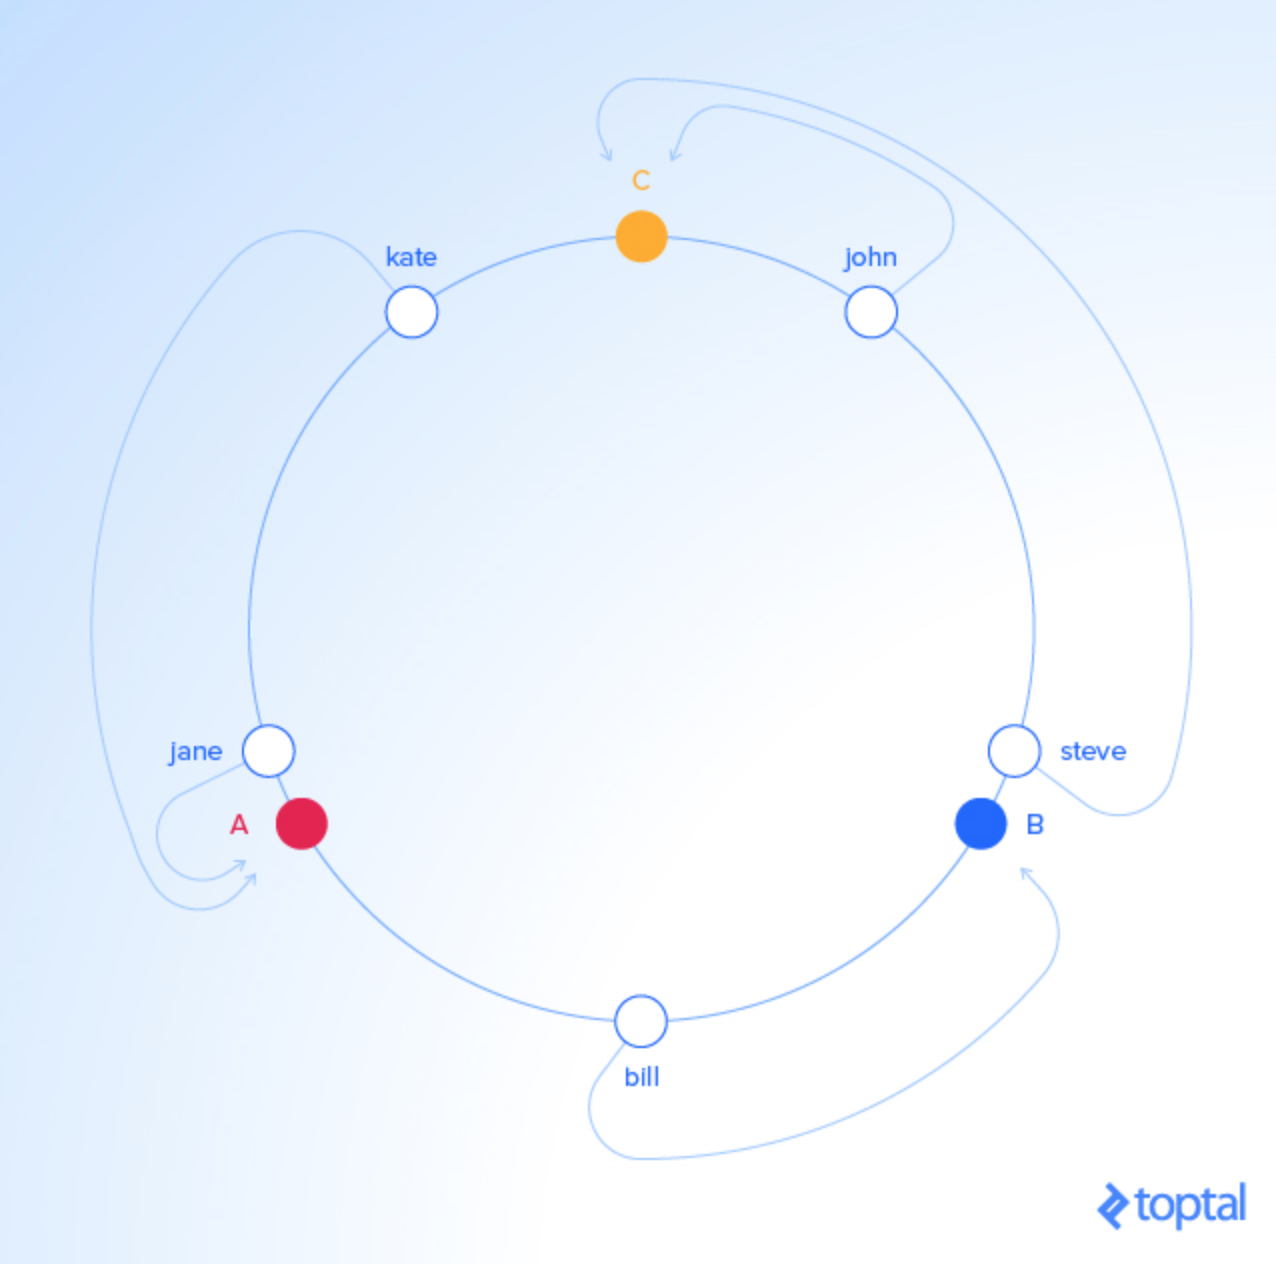
\includegraphics[width=0.55\textwidth]{thesis/figures/hashring.png}  
            \caption{Hash ring example (letters mark the nodes, names mark the keys) \cite{ConsistentHashing}.}
            \label{ConsistentHashingImage1}
        \end{figure}
        
        To be more consistent and distribute keys evenly among nodes, we can assign nodes not to one but to many places on the hash ring (Figure~\ref{ConsistentHashingImage2}).
        The number of one node keys, known as \textit{weight}, depends on the situation and may be different for each node depending of its capabilities (\textit{heterogeneity}). 
        Thanks to this solution we can easily add or remove nodes from the system and only $\frac{K}{n}$ keys need to be remapped, where $K$ stands for the number of keys and $n$ for the number of nodes.
        
        \begin{figure}[ht]
            \centering
                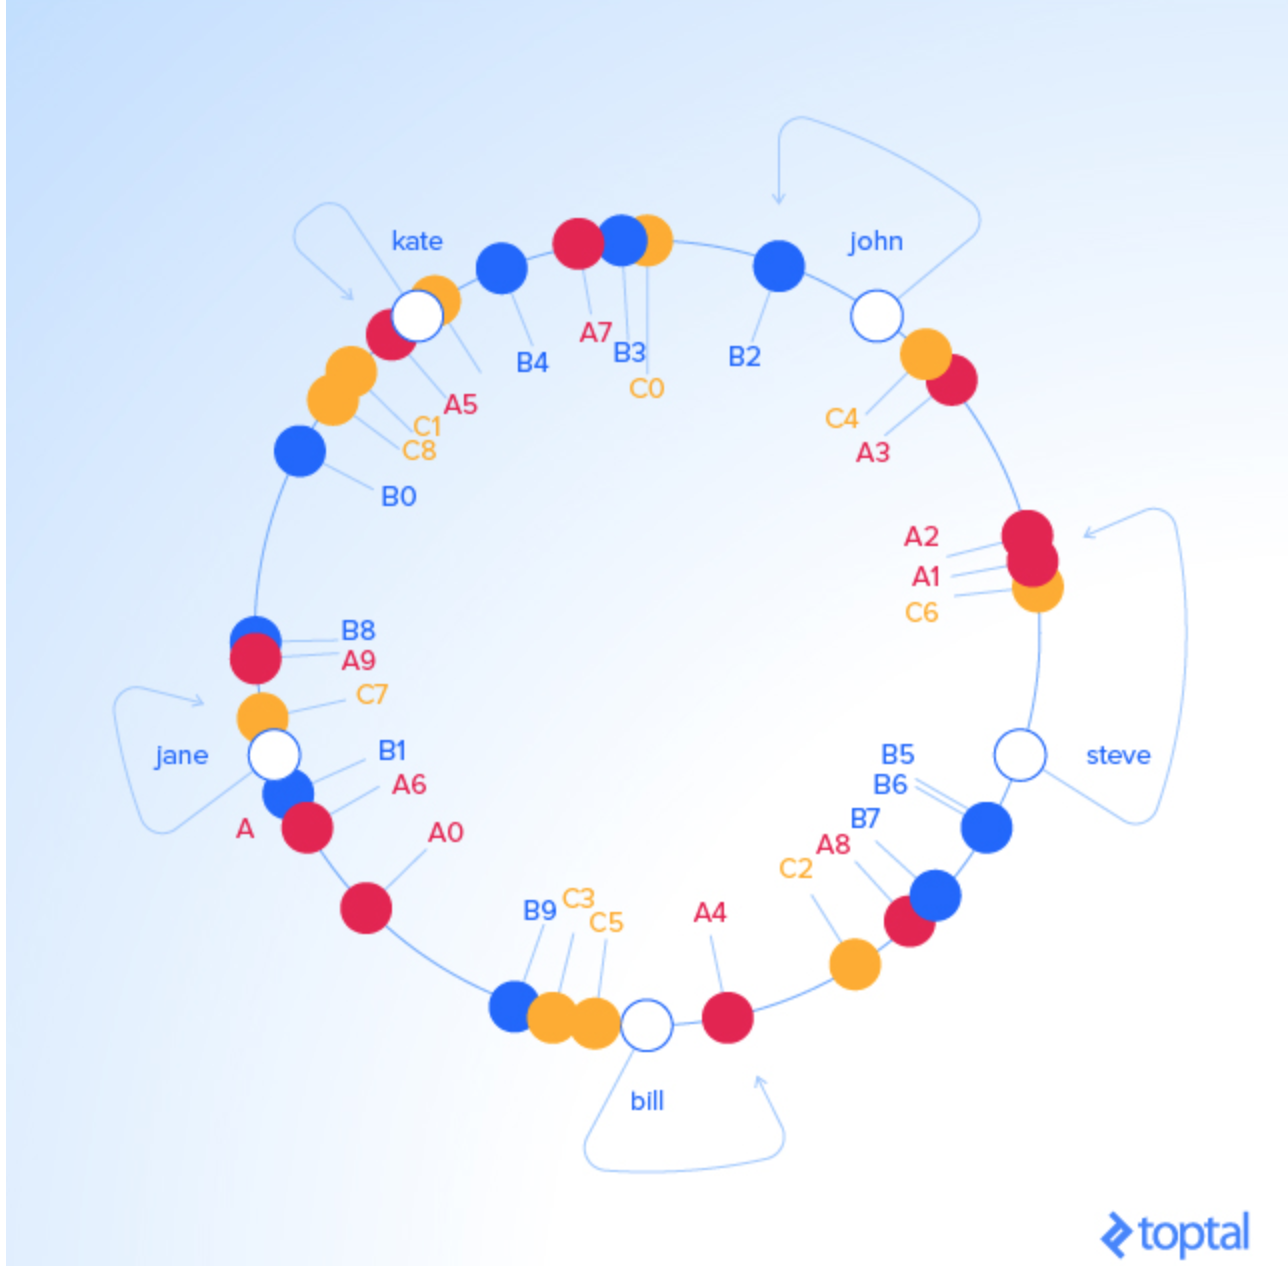
\includegraphics[width=0.55\textwidth]{thesis/figures/vnodes.png}
            \caption{Hash ring example with many node replicas (letters mark the nodes, names mark the keys) \cite{ConsistentHashing}.}
            \label{ConsistentHashingImage2}
        \end{figure}
        
    \subsection{Replication} 
        Since distributed systems can fail at any time we need to store data in a way that allows us to cope well with machine crashes. Storing any data item only on one node means that the data might be lost if the node crashes. Hence, data needs to be replicated. In order to specify on how many nodes each data item is to be replicated we define a configuration parameter called the \textit{replication factor}. 
        
        Consistent hashing can be easily extended to account for multiple replicas of each data item. To this end, for every node a full copy of its locally stored data is also kept on the neighbouring nodes (when looking clockwise). The total number of the replicas that store the same data depends on the replication factor. In consequence, when the first node on the ring that stores some data becomes unavailable and does not repond to the client's queries, the requests can be send to the next node on the ring. When a node crash is detected, the data maintained by this node (which are still available through the other nodes) are further replicated in order to satisfy the desired replication level.
        
    \subsection{Used programming libraries}
        The first version of \DHTS used the \emph{Seastar} networking library \cite{Seastar}. The final version uses \Asio\cite{Asio}. Below we describe both libraries and explain why we ultimately used the latter.
    
        \subsubsection{Seastar}
            \Seastar is an event-driven framework which allows the programmer to write non-blocking, asynchronous code. \Seastar is optimized for complex server applications running on modern multi-core machines. Among others, \Seastar features the share-nothing programming model and a custom networking stack, which enables direct access to the network interface buffers on a certain class of hardware. \Seastar's API is based on \textit{futures} and \textit{continuations}, thus providing the asynchronous programming model. The most well known use case of \Seastar is ScyllaDB\cite{ScyllaDB}, a highly optimized C++-based drop-in replacement for Apache Cassandra\cite{Cassandra}, a very popular NoSQL data store.
            
            The \Seastar framework caused many problems with development. The description of the building and configuration process provided by \Seastar's authors is complicated and incomplete. \Seastar's  documentation is missing some crucial informationa and many functions or classes are not described, e.g.: \texttt{engine} class. The provided code samples do not allow one to easily build a basic working client-server application.
            
            We tried to conduct the initial tests of \Seastar on Ubuntu 18.04 LTS, one of the officially supported Linux distributions. Due to the never ending problems in deploying the library, we eventually migrated to Fedora 27, which proved much easier to configure properly. 
            
            Later in the development process, we encountered a problem which proved to hard to overcome. The problem occurred when we tried to merge PHT with our \Seastar-based middleware. During initialisation, the \Seastar framework performed changes of the \texit{hugepages} \cite{Hugepages}, which made PMDK unable to allocate memory.
            
        \subsubsection{Boost Asio}
            \Asio is a C++ networking library which is mainly designed for the asynchronous programming model. \Asio is a part of the \textit{Boost} library, and it offers:
            \begin{itemize}
                \item portability -- support for commonly used operating systems,
                \item scalability -- scaling to thousands of concurrent connections,
                \item efficiency -- minimisation of data copying,
                \item support for IPv4 and IPv6,
                \item support for SSL connections.
            \end{itemize}
            \Asio provides support for basic network protocols like TCP, UDP and ICMP. Moreover, it also features the support for a low-level interface based on BSD socket. Depending on platform, \Asio uses different low-level networking mechanisms: \texttt{epoll} on Linux 2.6, \texttt{kqueue} on FreeSBD/MacOSX and \texttt{Overlapped IO} on MS Windows.
            
            We developed and tested \DHTS on Linux, which means that our implementation relied on \texttt{epoll} \cite{Epoll}. \texttt{epoll} (which stands for \emph{event poll}) allows an application to efficiently monitor multiple file descriptors/sockets to check whether any input or output action can be performed on any on them. This way the application is able to asynchronously read data from sockets.

\chapter{Own work}

\section{NVM-enabled hashtable}

\subsection{Tests}

    To ensure that our hashtable works correctly, we developed a range of unit tests. As previously stated, we used the GoogleTest library. We decided to split our tests into two categories: logic and perfomance.
    
    Logic tests try to verify the correctness of basic operands used in our hashtable: insert, get, remove and iterate. We run them on two instances of hashtable: integer and string type. In first test we add a number of elements with known sum. Then we start iterating through hashmap, at the same time summing elements. At the end with assert we check for equality of those two sums. Next tests concentrates on insert, get and remove functionalities. We decided to verify them both in single such as multithread mode (using 8 threads), where one thread inserts 100 thousand elements. After completing the addition, in one test case we try to get previously added elements, while in the second one we try to remove them. For each element we compare received value with added one using an assert.
    
    In performance tests we concentrated on comparing the effectiveness of our hashtable with \textit{unordered\_map} from std namespace. We measured time for 8 threads to insert, get and remove elements. We conducted the same calculations for respectively 16, 8, 4, 2 and 1 thread.
    
    
    

        
    

% Rozdziały dokumentujące pracę własną studenta: opisujące ideę, sposób lub metodę 
% rozwiązania postawionego problemu oraz rozdziały opisujące techniczną stronę rozwiązania 
% --- dokumentacja techniczna, przeprowadzone testy, badania i uzyskane wyniki. 

% Praca musi zawierać elementy pracy własnej autora adekwatne do jego wiedzy praktycznej uzyskanej w
% okresie studiów. Za pracę własną autora można uznać np.: stworzenie aplikacji informatycznej lub jej
% fragmentu, zaproponowanie algorytmu rozwiązania problemu szczegółowego, przedstawienie projektu 
% np.~systemu informatycznego lub sieci komputerowej, analizę i ocenę nowych technologii lub rozwiązań
% informatycznych wykorzystywanych w przedsiębiorstwach, itp. 

% Autor powinien zadbać o właściwą dokumentację pracy własnej obejmującą specyfikację założeń i 
% sposób realizacji poszczególnych zadań
% wraz z ich oceną i opisem napotkanych problemów. W przypadku prac o charakterze 
% projektowo-implementacyjnym, ta część pracy jest zastępowana dokumentacją techniczną i użytkową systemu. 

% W pracy \textbf{nie należy zamieszczać całego kodu źródłowego} opracowanych programów. Kod źródłowy napisanych
% programów, wszelkie oprogramowanie wytworzone i wykorzystane w pracy, wyniki przeprowadzonych
% eksperymentów powinny być umieszczone na płycie CD, stanowiącej dodatek do pracy.

% \section*{Styl tekstu}

% Należy\footnote{Uwagi o stylu pochodzą częściowo ze stron Macieja Drozdowskiego~\cite{mdro}.} 
% stosować formę bezosobową, tj.~\emph{w pracy rozważono ......, 
% w ramach pracy zaprojektowano ....}, a nie: \emph{w pracy rozważyłem, w ramach pracy zaprojektowałem}. 
% Odwołania do wcześniejszych fragmentów tekstu powinny mieć następującą postać: ,,Jak wspomniano wcześniej, ....'', 
% ,,Jak wykazano powyżej ....''. Należy unikać długich zdań. 

% ,,Ilość'' i ,,liczba''. Proszę zauważyć, liczba dotyczy rzeczy policzalnych, np.~liczba osób, liczba zadań, procesorów. 
% Ilość dotyczy rzeczy niepoliczalnych, np.~ilość wody, energii. Należy starać się wyrażać precyzyjnie, tj.~zgodnie 
% z naturą liczonych obiektów.\footnote{(DW) Według wytycznych Rady Języka Polskiego obie formy są dopuszczalne
% zarówno do obiektów policzalnych, jak i niepoliczalnych. W tekstach technicznych warto być jednak precyzyjnym.}

% Niedopuszczalne są zwroty używane w języku potocznym. W pracy należy używać terminologii informatycznej, która ma 
% sprecyzowaną treść i znaczenie. Nie należy używać ,,gazetowych'' określeń typu: 
% silnik bazy danych, silnik programu, maszyna skryptowa, elektroniczny mechanizm, mapowanie, string, gdyż nie wiadomo 
% co one właściwie oznaczają. 

% Niedopuszczalne jest pisanie pracy metodą \emph{cut\&paste}, bo jest to plagiat i dowód intelektualnej indolencji autora.
% Dane zagadnienie należy opisać własnymi słowami. Zawsze trzeba powołać się na zewnętrzne źródła. 



\chapter{Conclusion}

% Zakończenie pracy zwane również Uwagami końcowymi lub Podsumowaniem powinno zawierać ustosunkowanie
% się autora do zadań wskazanych we wstępie do pracy, a w szczególności do celu i zakresu pracy oraz
% porównanie ich z faktycznymi wynikami pracy. Podejście takie umożliwia jasne określenie stopnia
% realizacji założonych celów oraz zwrócenie uwagi na wyniki osiągnięte przez autora w ramach jego
% samodzielnej pracy.

% Integralną częścią pracy są również dodatki, aneksy i załączniki np.~płyty CDROM
% zawierające stworzone w ramach pracy programy, aplikacje i projekty.


% All appendices and extra material, if you have any.
\cleardoublepage\appendix%
%\input{0a-appendix.tex}

% Bibliography (books, articles) starts here.
\bibliographystyle{alpha}{\raggedright\sloppy\small\bibliography{bibliography}}

% Colophon is a place where you should let others know about copyrights etc.
\ppcolophon

\end{document}
